\documentclass{article}
\usepackage{graphicx} % Required for inserting images
\usepackage{amsmath}
\usepackage{amsfonts}
\usepackage{subcaption}
\usepackage{hyperref}
\usepackage{epigraph}

\usepackage[left=3cm, right=3cm, top=2cm, bottom=2cm]{geometry}
\usepackage[style=numeric]{biblatex}
\addbibresource{refs.bib}

\title{[MVA] - Rapport de stage}
\author{Mathis Reymond}
\date{April 2024}

\begin{document}

\maketitle
\epigraph{Goodhart's law}{When a metric becomes a target, it ceases to be a good metric.}

\section{Introduction}

Continual learning is a machine learning paradigm that focuses on the ability of a model to learn and adapt to new information over time, without forgetting previously learned knowledge. It is particularly relevant in scenarios where data is non-stationary or arrives in a sequential manner. By leveraging techniques such as online learning, regularization, and knowledge distillation, continual learning enables models to continuously update their knowledge and improve performance as new data becomes available.

\subsection{Initial project}
\subsubsection{Project statement}

In this context, the aim of the project was initialy stated as follows:

\begin{quote}
    \itshape
    Catastrophic forgetting is a major challenge in continual learning systems, where a neural network needs to adapt to new tasks that differ from what it has previously learned. To tackle this, experts have devised strategies to either keep the neural network's critical weights intact or use generative models to refresh the network's memory of past tasks. However, these methods aren't perfect for hardware implementation due to their additional memory demands or the need for a separate network that constantly rehearses past information.

    Meanwhile, we understand that a system's architecture significantly impacts its ability to generalize knowledge. Enter Gradmax \cite{gradmax}, an innovative algorithm that simultaneously optimizes a network's structure and weights, and smartly allocates neurons for new tasks without disrupting existing knowledge. This method is memory and computation efficient, making it suitable for hardware applications. But it does require hardware capable of dynamically adjusting its architecture to integrate new neurons as needed. Our recent work has led to a flexible hardware architecture, Mosaic \cite{mosaic}, with multiple cores that can rearrange their connections in real-time.

    The aim of this project is to explore the integration of Gradmax with our dynamic 'Mosaic' architecture. We plan to approach this by factoring hardware limitations into the optimization process. In addition, we're considering the development of a gating network within this architecture that determines the optimal timing for assigning tasks to newly added neurons. This could leverage cutting-edge techniques like Mixture of Expert models \cite{DME}.
\end{quote}

\noindent
Let's dissect this project statement to understand the main objectives and challenges it encapsulates.\\
\\
\noindent
\textbf{Computational costs.} The project aims to address the computational costs associated with continual learning methods. Thus we expect to have a way to measure this cost, employ as figure of merit or intregrate it to the optimization process and to compare it to the cost of other methods.\\
\\
\noindent
\textbf{Continual learning approach.} Litterature categorizes continual learning approaches into three main categories: rehearsal, regularization, and architectural. However in the process of taking into account the computational costs, we will explore the architectural approach.\\
\\
\noindent
\textbf{Gradmax} Gradmax is a method designed for learning on a single task. Thus this project invites to extend it to continual learning. \\
\\
\noindent
\textbf{Mosaic} In the process of adapting Gradmax method to the continual learning framework, we will have to consider the hardware constraints of the Mosaic architecture.




\subsubsection{Major issues}

In the very beginning of the project, we faced two major issues. The first one is a consequence of Gradmax paper misleading introduction. Indeed, in the very first paragraph of the paper, the authors introduces :
\begin{quote}
    \itshape
    \centering
    Searching for the best architecture for a given task is an active research area with diverse approaches.[...] Most of these approaches are costly, as they require large search spaces or large architectures to start with. In this work we consider an alternative approach.
\end{quote}

\noindent
The genuine expectation regarding the work following such an introduction is that the authors will provide an inovative method that factorizes architecture search in the optimization process of learning a task while avoiding to train numerous high-size architectures, which is computationally expensive.\\

\noindent
However, contrary to expectations, GradMax falls short at enabling neural architecture optimization. The method consists in growing a network from a root architecture to a predetermined target architecture, by adding neurons to it through training epochs. It focuses on the initialization of added neurons (the \textit{how}), neglecting the crucial questions of \textit{when} and \textit{where} to add them, which are deferred for future research. In the paper, the decisions regarding \textit{where} and \textit{when} to add neurons are predetermined and take the form of a schedule established. Consequently, it's challenging to conclude that the GradMax framework effectively enables architecture optimization for growing artificial neural networks.\\

\noindent
Additionaly, authors do not consider the computational cost of their method in the rest of the paper. This is a major issue as the project was initially designed to reduce the computational cost of continual learning methods.

\subsubsection{Additional hurdles}

As a general concept, we considere that continual learning referes to the ability of a model to learn and adapt to new information over time, without forgetting previously learned knowledge. However, this wide definition encompasses a variety of scenarios.
First, it can be the case that there is no explicit task boundary, and the model must continuously adapt to new data without any indication of when a new task begins. This is known as incremental learning. Second, the model may be presented with a sequence of tasks, each with its own training data and objectives. In this case, the model must learn each task sequentially and adapt to new tasks without forgetting the previous ones, which is known as sequential learning. Third, the model may be presented with a series of tasks that are related or have some shared structure. In this case, the model must leverage this shared structure to learn new tasks more efficiently. This is known as multitask learning.

But even after this specification, ambiguities persist. For instance when it comes to sequential learning, some frameworks assume that the model is knows when a new task arrives, whereas others do not make this assumption.

\subsection{Revised project}


\section{Approaches explored}
\subsection{LoRA}


\subsection{Growth in continual learning}
\subsubsection{Motivating growth exploration}


Trying to taclke the questions of where and when to grow neurons in the framework of GradMax, that is, starting with a root architecture and converging to a target architecture, it can be interesting to assess whether or not the way we grow the architecture toward this target architecture matters. For example, we can considere a simple two-hidden layer architecture, and grow it by adding neurons to the first hidden layer first, then to the second hidden layer, or the other way around. So the order we add neurons to each layer define a path. And we can ask ourselves if some paths are more efficient than others.

\begin{figure}[htbp]
    \centering
    \begin{subfigure}[b]{0.29\textwidth}
        \centering
        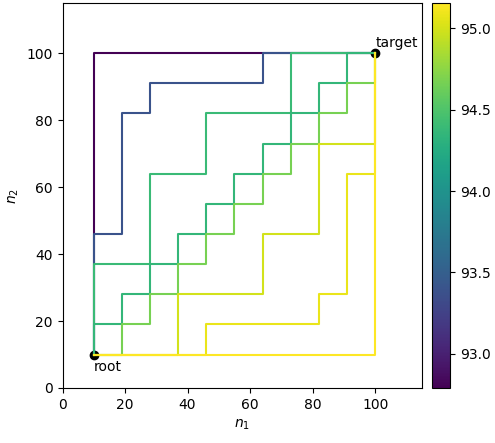
\includegraphics[width=0.9\textwidth]{imgs/pathes_MNIST_gradmax_2024_05_02_15_03_12.png}
        \caption{Average test accuracy achieved by following each paths to grow the network, accross 5 trials}
        \label{fig:MNIST_gradmax_pathes}
    \end{subfigure}
    %\hfill
    \begin{subfigure}[b]{0.29\textwidth}
        \centering
        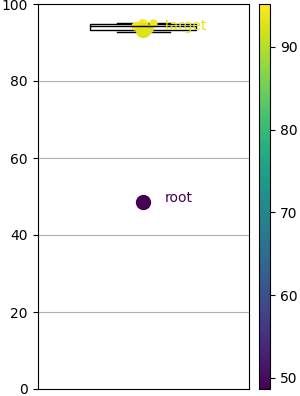
\includegraphics[width=0.6\textwidth]{imgs/box_plot_MNIST_gradmax_2024_05_02_15_03_13.png}
        \caption{Average test accuracies of the paths, the root model and the taregt model, accross 5 trials}
        \label{fig:MNIST_gradmax_box_plot}
    \end{subfigure}
    
    \vspace{0.5cm}
    
    \begin{subfigure}[b]{0.5\textwidth}
        \centering
        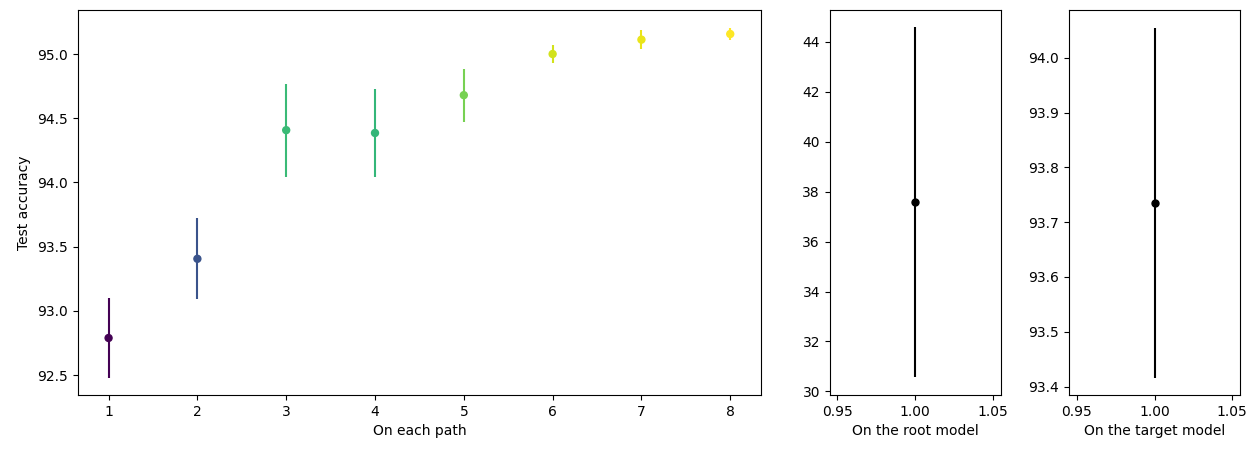
\includegraphics[width=\textwidth]{imgs/statistical_reliability_MNIST_gradmax_2024_05_02_15_03_12.png}
        \caption{Average test accuracy across 5 trials, with standard deviation}
        \label{fig:MNIST_gradmax_statistical_reliability}
    \end{subfigure}
    \caption{Results on MNIST with GradMax initialization}
    \label{fig:subfigures}
\end{figure}

To do so, we set the root network (RN) to be a two-hidden-layer MLP with 10 neurons on each layer, and the target network (TN) to be a two-hidden-layer MLP with 100 neurons on each layer. As reference for comparison, we train both RN and TN on 300 batch MNIST batches, each of which is of size 128, for 3 epochs. We use Adam optimizer with learning rate equal to $5\times10^{-3}$, and mean squarred error loss function. We repeat this process 5 times for statistical reliability. See \ref{fig:MNIST_gradmax_statistical_reliability} for the results.

Then, in the processus of growing RN toward TN through the training process, we define schedules. Each schelule consists 20 growth step. 10 of these growth steps consist in adding 9 neurons to the first and the other 10 growth steps consist in adding 9 neurons the second hidden layer. Thus, the only way two schedules differ from each other is this order it plans to grow each layer. As for training RN and TN, the growing process occurs while training on 300 batch MNIST batches, each of which is of size 128, for 3 epochs. Overall, each growth of 10 neurons happens once every We use Adam optimizer with learning rate equal to $5\times10^{-3}$, and mean squarred error loss function.

That being said, we can see that the path we choose to grow the network has a significant impact on the final test accuracy. In particular, the path that consists in adding neurons to the first hidden layer first, then to the second hidden layer, seems to be the most efficient. 

Thus, exploring neurogeneis makes sense in the context of traditional learning (on a single task). However, what we want to do is to adapt this to a contiual learning framework. That is, we want to grow the network  



\subsection{EWC}


Issues with the fundational paper itself :
\begin{itemize}
    \item No code avaiable
    \item No specification of the number of $\lambda$ parameters
    \item No specification of the values of the $\lambda$ parameters
    \item Mismatch between figure and references to figures
\end{itemize}

\noindent
Issues with the approach :
\begin{itemize}
    \item Ranks on paperwithcode benchmarks : $\frac{5}{6},\frac{13}{15},\frac{6}{8},\frac{6}{6},\frac{3}{7}$, so the approach falls just above the first quintile, ranking on average 22th out of 100 approaches. But when we read the paper, it feels like continual learning is solved.
    \item Redundancy
    \item 2 to 1 pollution
    \item 1 to 2 pollution
    \item Too much hyper parameters (lambda(s))
    \item Fact that no matter how hard you try, every time you learn a new task, you do hurt knowledge about the previous tasks. So from the very beginning, the approach is doomed to be very limited... the only way to save the face is to overfit with loads of HPs.
\end{itemize}



\subsection{Conclusions we can draw from these attempts}
\subsubsection{Limitation of approaches}


As a very general principle, the problem with these approaches in the context of continual learning is that
\begin{quote}
    \itshape
    \centering
    Improving on task 2 mean regressing on task 1, and reciprocally
\end{quote}

\noindent
Which implies that performing continual learning in such a way requires to perform trade-offs. And the most convenient way one performs trade-offs in deep learning is through hyperparameters.

\vspace{0.5cm}

\noindent
We often assume that it is fine to attempt somewhat limited approaches because improvements are achieved by building on failed attempts. This is true for incremental improvements, typically made by engineers through the combination and optimization of previous work. However, researchers aim for disruptive improvements by stepping back from the current state of the art to identify what is arbitrary, poorly motivated, or inherently limited in current approaches.

\vspace{0.5cm}

\noindent
Let's assume we are given $I$ tasks indexed by the set $\{1,2,...,I\}$. We define a neural network as the set of its parameters
\begin{align}
    \phi = \left\{\left\{w_{l,m,n}\right\}\right\} \in \mathbb{R}^{L+1,N_{l-1},N_{l}}
\end{align}

Let's define $\mathbb{W}_i$ the set of protected weights for task $i$ by 
\begin{align}
    \mathbb{W}_i
\end{align}

\vspace{0.5cm}

\noindent
To this regard, as a general concept, we can control :
\begin{itemize}
    \item how the added neurons react to new task samples
    \item how the old neurons react to new task samples
    \item (depending on the approach) how the old neurons react to previous tasks samples
\end{itemize}

However, we have absolutely no control over the way the added neurons react to previous tasks samples because :
\begin{itemize}
    \item we have no acces to previous tasks samples
    \item we are not using any rehearsal strategy
    \item we do not intend to encode any information about the specificity of previous tasks in the weights 
\end{itemize}

So our very last hopes without memory are :
\begin{itemize}
    \item to parametrize/constrain the weights so that they encode task information
\end{itemize}

Interestingly, these questions and remarks we have been objecting to ourselves about fundations of our approach applies to several other approaches including :
\begin{itemize}
    \item regularization approaches such as EWC, Hessian and Bayesian approaches
    \item our LoRA approach
    \item neural growth approaches (whether initialization is done randomly, through GradMax or TINY)
    \item use of distincts neural networks for each task
\end{itemize}

However, when reading papers about these approaches we have the general feeling that continual learning is a solved problem whereas we argued that they are not adressing continual learning. While they have no information about previous tasks, these approaches can only positive results by performing trade offs between the total number of tasks in the benchmark, how much you forget about the previous tasks and how much you can learn about the new one at hand. That is, these approaches heavily rely on hyperparameter optimization.


So in a nutshell, these approaches succeed at solving one specific continual learning benchmark at a time. None of these approaches can perform well on a new benchmark without going through a new heavy hyperparameter optimization process. So, can we really considere them as general continual learning approaches ? Because there seem to a close ressemblance to overfitting ; a hyper-overfitting.

Would we need to need to define a validation set of benchmarks ? And require every approaches to be able to run on test benchmarks with none of few hyperparameter updates ?


\subsubsection{Lack of specificity and definitions}

In addition to the previous

no definition of :
- overfitting on a benchmark
    - define and measure the hyper parameter importance (or cost) of any given approach, to quantify overfitting
- task
- similarity between tasks

\nocite{*}
\printbibliography


\section*{Appendix}
\subsection{Other results for motivating exploration of growth paths}

% MNIST random
\begin{figure}[htbp]
    \centering
    \begin{subfigure}[b]{0.29\textwidth}
        \centering
        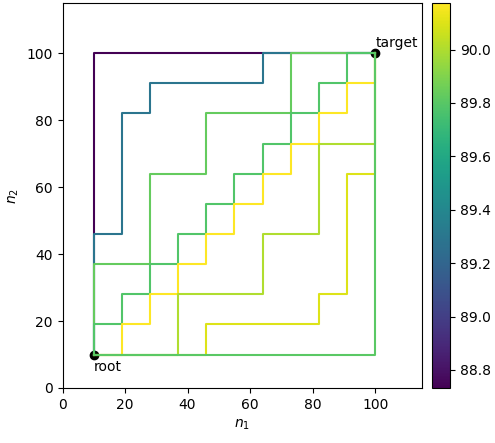
\includegraphics[width=0.9\textwidth]{imgs/pathes_MNIST_random_2024_05_02_14_52_58.png}
    \end{subfigure}
    %\hfill
    \begin{subfigure}[b]{0.29\textwidth}
        \centering
        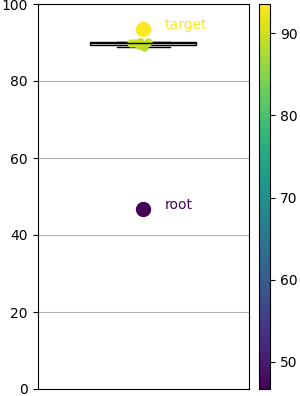
\includegraphics[width=0.6\textwidth]{imgs/box_plot_MNIST_random_2024_05_02_14_52_58.png}
    \end{subfigure}
    
    \vspace{0.5cm}
    
    \begin{subfigure}[b]{0.5\textwidth}
        \centering
        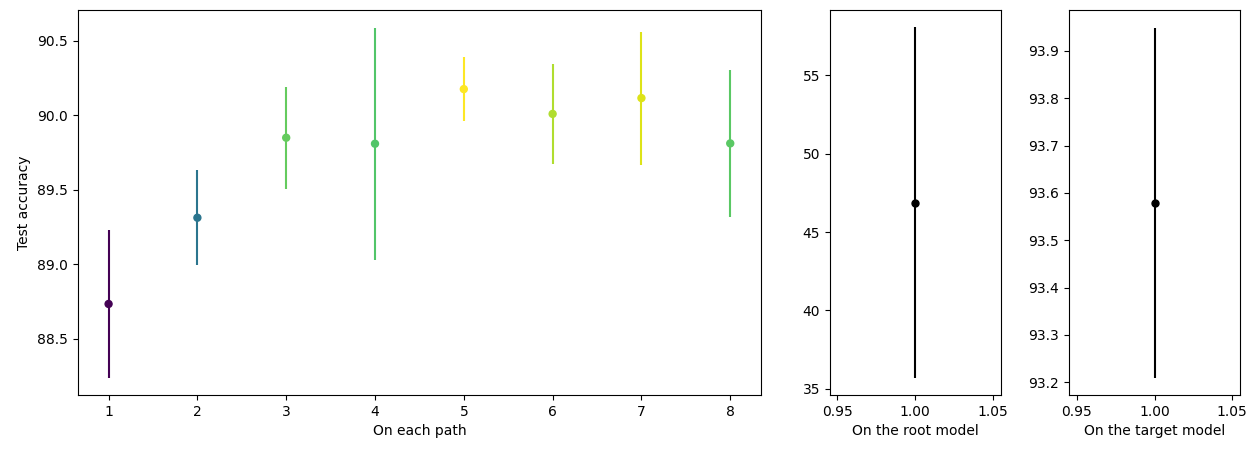
\includegraphics[width=\textwidth]{imgs/statistical_reliability_MNIST_random_2024_05_02_14_52_58.png}
    \end{subfigure}
    \caption{Results on MNIST with random initialization}
\end{figure}

% FMNIST random
\begin{figure}[htbp]
    \centering
    \begin{subfigure}[b]{0.29\textwidth}
        \centering
        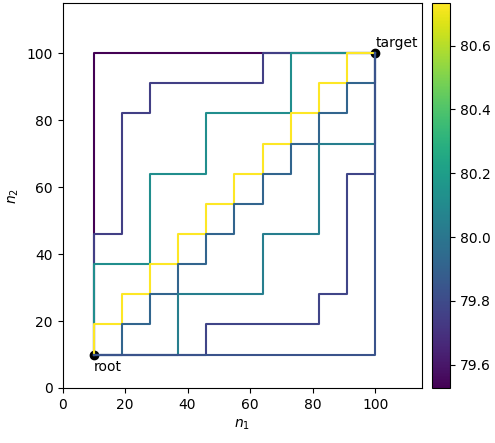
\includegraphics[width=0.9\textwidth]{imgs/pathes_FNIST_random_2024_05_02_15_13_26.png}
    \end{subfigure}
    %\hfill
    \begin{subfigure}[b]{0.29\textwidth}
        \centering
        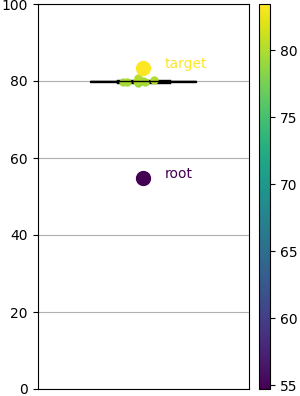
\includegraphics[width=0.6\textwidth]{imgs/box_plot_FNIST_random_2024_05_02_15_13_27.png}
    \end{subfigure}
    
    \vspace{0.5cm}
    
    \begin{subfigure}[b]{0.5\textwidth}
        \centering
        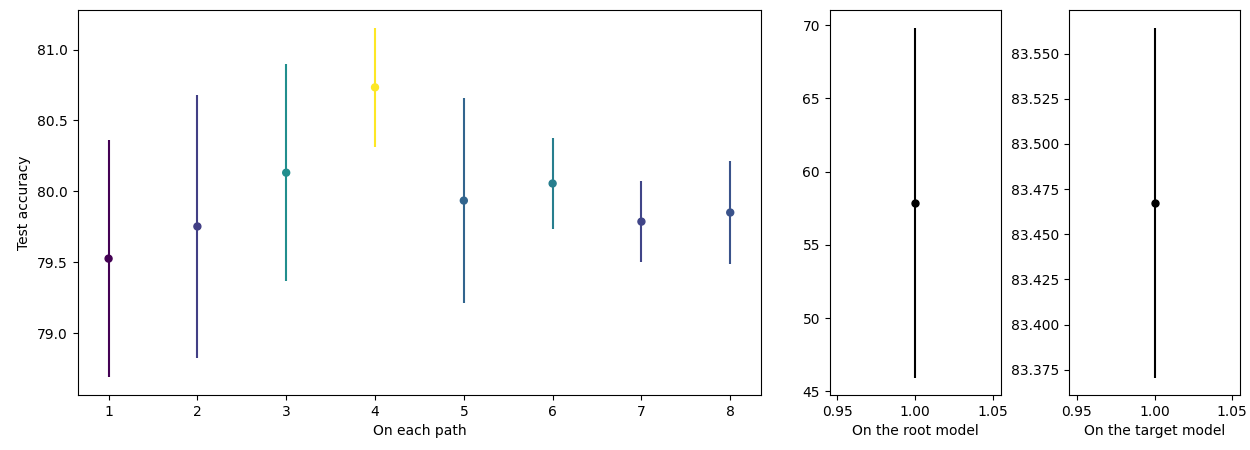
\includegraphics[width=\textwidth]{imgs/statistical_reliability_FNIST_random_2024_05_02_15_13_27.png}
    \end{subfigure}
    \caption{Results on FMNIST with random initialization}
\end{figure}

% FMNIST gradmax
\begin{figure}[htbp]
    \centering
    \begin{subfigure}[b]{0.29\textwidth}
        \centering
        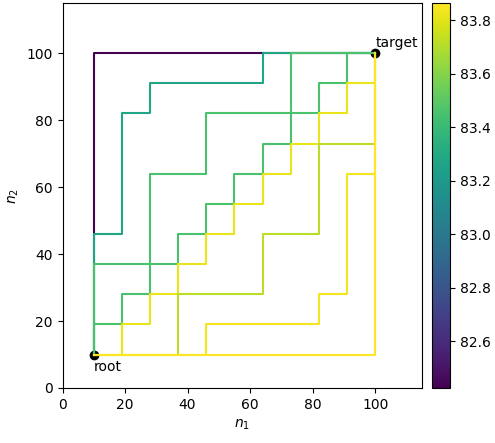
\includegraphics[width=0.9\textwidth]{imgs/pathes_FMNIST_gradmax_2024_05_02_15_23_40.png}
    \end{subfigure}
    %\hfill
    \begin{subfigure}[b]{0.29\textwidth}
        \centering
        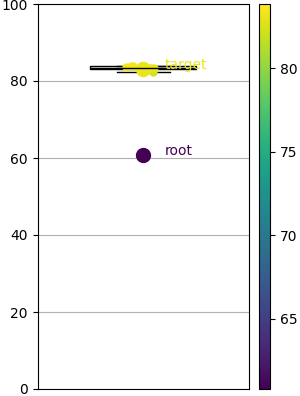
\includegraphics[width=0.6\textwidth]{imgs/box_plot_FMNIST_gradmax_2024_05_02_15_23_40.png}
    \end{subfigure}
    
    \vspace{0.5cm}
    
    \begin{subfigure}[b]{0.5\textwidth}
        \centering
        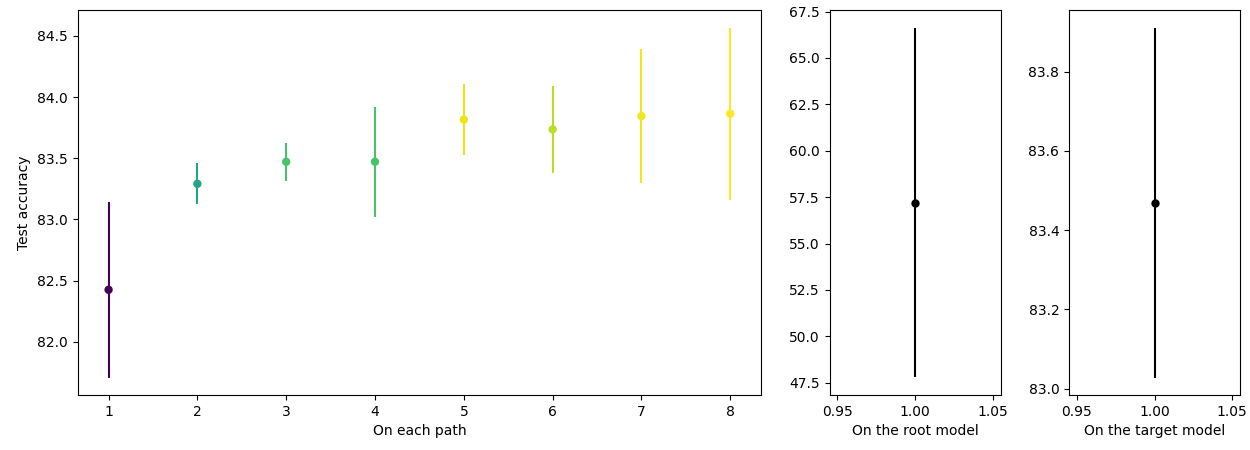
\includegraphics[width=\textwidth]{imgs/statistical_reliability_FMNIST_gradmax_2024_05_02_15_23_40.png}
    \end{subfigure}
    \caption{Results on FMNIST with gradmax initialization}
\end{figure}

% CIFAR10 random
\begin{figure}[htbp]
    \centering
    \begin{subfigure}[b]{0.29\textwidth}
        \centering
        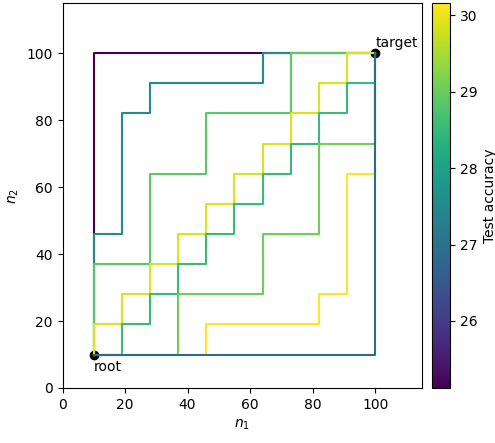
\includegraphics[width=0.9\textwidth]{imgs/pathes_CIFAR10_random_2024_05_02_15_49_40.png}
    \end{subfigure}
    %\hfill
    \begin{subfigure}[b]{0.29\textwidth}
        \centering
        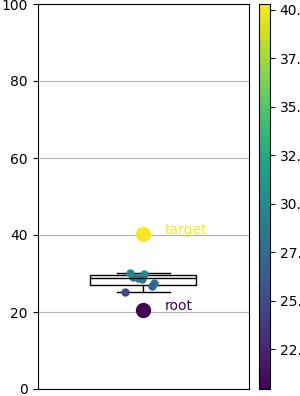
\includegraphics[width=0.6\textwidth]{imgs/box_plot_CIFAR10_random_2024_05_02_15_49_41.png}
    \end{subfigure}
    
    \vspace{0.5cm}
    
    \begin{subfigure}[b]{0.5\textwidth}
        \centering
        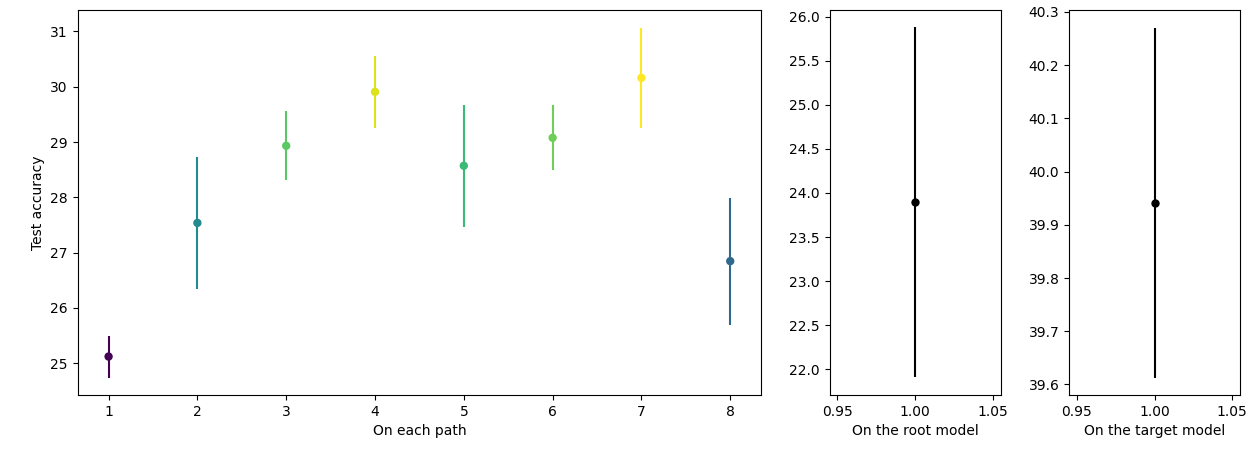
\includegraphics[width=\textwidth]{imgs/statistical_reliability_CIFAR10_random_2024_05_02_15_49_40.png}
    \end{subfigure}
    \caption{Results on CIFAR10 with random initialization}
\end{figure}

% CIFAR10 gradmax
\begin{figure}[htbp]
    \centering
    \begin{subfigure}[b]{0.29\textwidth}
        \centering
        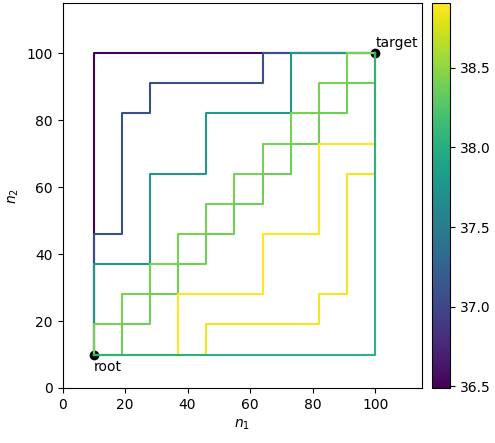
\includegraphics[width=0.9\textwidth]{imgs/pathes_CIFAR10_gradmax_2024_05_02_16_13_51.png}
    \end{subfigure}
    %\hfill
    \begin{subfigure}[b]{0.29\textwidth}
        \centering
        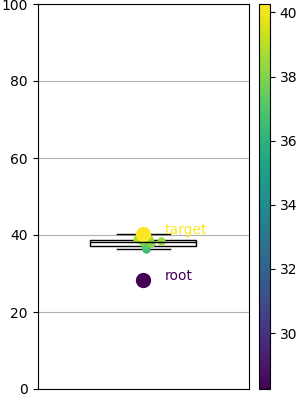
\includegraphics[width=0.6\textwidth]{imgs/box_plot_CIFAR10_gradmax_2024_05_02_16_13_51.png}
    \end{subfigure}
    
    \vspace{0.5cm}
    
    \begin{subfigure}[b]{0.5\textwidth}
        \centering
        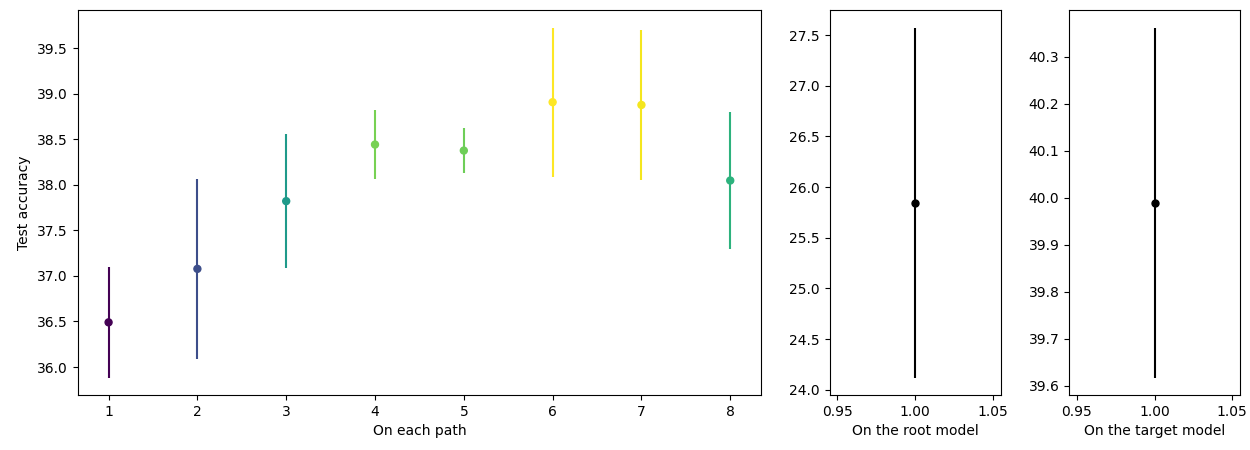
\includegraphics[width=\textwidth]{imgs/statistical_reliability_CIFAR10_gradmax_2024_05_02_16_13_51.png}
    \end{subfigure}
    \caption{Results on CIFAR10 with gradmax initialization}
\end{figure}

\end{document}
